% !TeX spellcheck = de_DE
\documentclass{uebung_cs}
\usepackage{algo221}
\uebung{1}{}{}
\blattname{Übungen zu Woche 1: Einführung und All Pairs Shortest Paths}
%%%%%%%%%%%%%%%%%%%%%%%%%%%%%%%%%%%%%%%%%%%%%%%%%%%%%%%%%%%%%%%%%%%%%%%%%%%%
\begin{document}

Das Übungsblatt enthält alle empfohlenen Lernaktivitäten für die aktuelle Woche.

\begin{itemize}
\item \textbf{Dienstag 8--10.} Bearbeite jetzt die Übungen im Abschnitt \textbf{Dienstag}. Sprich mit anderen Studis! Frag das Vorlesungsteam um Hilfe!
\item \textbf{Heimarbeit bis Mittwoch 17:00.}
\begin{itemize}
\item 
Schau die Videos an und lies [Erickson, Kapitel 9.1, 9.2, 9.5--9.8]. Mach dir Notizen, wenn du etwas nicht verstanden hast!
\item Bearbeite die \emoji{seedling}-Aufgabe in \href{https://moodle.studiumdigitale.uni-frankfurt.de/moodle/course/view.php?id=2241}{Moodle}. (Feste Abgabefrist!)
\item Lies den Aufgabentext aller Übungsaufgaben.
\item Bearbeite die Übungsaufgaben im Abschnitt \textbf{Donnerstag}. Wenn du für mehr als 30 Minuten stecken bleibst, geh zur nächsten Übungsaufgabe.
\end{itemize}
\item \textbf{Donnerstag 8--10.} Bearbeite jetzt die Übungen, die du noch nicht lösen konntest. Sprich mit anderen Studis! Frag das Vorlesungsteam um Hilfe!
\item \textbf{Heimarbeit bis Freitag 17:00:} Gib deine Lösung zur aktuellen \emoji{star}-Aufgabe in \href{https://moodle.studiumdigitale.uni-frankfurt.de/moodle/course/view.php?id=2241}{Moodle} ab. (Feste Abgabefrist!)
\end{itemize}

\section*{Dienstag}

\begin{aufgabe}[Orga]\
  \begin{enumerate}
    \item Lies alle Informationen auf der \href{https://tcs.uni-frankfurt.de/algo2/}{Webseite des Kurses}, auf der \href{https://moodle.studiumdigitale.uni-frankfurt.de/moodle/course/view.php?id=2241}{Moodle-Seite des Kurses}, und auf den \href{https://tcs.uni-frankfurt.de/algo2/organisation.pdf}{Organisationsfolien}.
    \item Melde dich jetzt mit einem Nickname deiner Wahl auf dem ALGO2 Discord-Server an. Den Link zum Discord-Server findest du in Moodle. (Es handelt sich hierbei \textbf{nicht} um den Discord-Server des Lernzentrums!)

    Nutze den Discord-Server im ganzen Semester, wenn du andere Studis zum Zusammenarbeiten suchst oder inhaltliche Fragen an das Vorlesungsteam hast.
  \end{enumerate}
\end{aufgabe}

\begin{aufgabe}[Coderunner ausprobieren]
    Löse jetzt die Aufgabe \enquote{Aufwärmübung: Coderunner ausprobieren} auf Moodle.
\end{aufgabe}

% \begin{aufgabe}[Pfannkuchensortierung]
%     Gegeben ist ein Stapel von $n$ Pfannkuchen verschiedener Größe.
%     Du musst die Pfannkuchen der Größe nach sortieren, sodass am Ende kleinere Pfannkuchen auf größeren Pfannkuchen liegen.
%     Die einzige erlaubte Operation ist ein \emph{flip}: Führe einen Pfannenwender unter die obersten $k$ Pfannkuchen für eine natürliche Zahl~$k$ ein und wende sie um.
%     \begin{enumerate}
%         \item Beschreibe einen Algorithmus, der einen beliebigen Stapel von $n$ Pfannkuchen mit $O(n)$ flips sortiert. Wie viele flips braucht dein Algorithmus im worst-case genau?
%         \item Für jede positive Zahl $n$, beschreibe einen Stapel mit $n$ Pfannkuchen, auf dem dein Algorithmus $\Omega(n)$ flips benötigt.
%     \end{enumerate}
% \end{aufgabe}

\begin{aufgabe}[Telefonnetzwerk]
    Gegeben sei ein Diagramm mit Schaltzentren und Verbindungen.
    Die Verbindungen können durch Kabel, Funk, oder Satellit realisiert werden.
    Wir modellieren dies, indem wir mit jeder Verbindung eine \emph{Bandbreite} und \emph{Kosten} assoziieren.
    \begin{enumerate}
        \item Gib einen Algorithmus an, der für zwei Schaltzentren $a$ und $b$ einen Verbindungsweg von $a$ nach $b$ ausrechnet, der die kleinsten Kosten verursacht.
        \item Die \emph{Bandbreite eines Verbindungsweg} ist die kleinste Bandbreite über alle einzelnen Verbindungen, die auf dem Weg auftauchen.
        Gib einen Algorithmus an, der für zwei Schaltzentren $a$ und $b$ einen Verbindungsweg von $a$ nach $b$ ausrechnet, der die größtmögliche Bandbreite hat.
    \end{enumerate}
\end{aufgabe}

\begin{aufgabe}[Puzzle der Woche: 99 Polizisten]\
  In einer Stadt arbeiten 99 Polizisten.
  Jeder Polizist ist entweder ehrlich oder korrupt, wobei die Mehrheit der Polizisten ehrlich ist.
  Finde mit weniger als 299 Fragen heraus, welches die korrupten Polizisten sind.
  
  Dabei wissen alle Polizisten, welche der Polizisten ehrlich und welche korrupt sind, aber nur ehrliche Polizisten antworten immer wahrheitsgemäß.
  Korrupte Polizisten lügen möglicherweise.
  Aus sicherheitsgründen können nur Fragen folgenden Typs gestellt werden: Du kannst einen Polizisten X fragen, ob Polizist Y korrupt ist.
  Die Antwort darauf lautet entweder \enquote{Y ist korrupt} oder \enquote{Y ist ehrlich}.

\end{aufgabe}

\section*{Donnerstag}

\begin{aufgabe}[APSP-Algorithmen anwenden]
  Gegeben sei der gerichtete und gewichtete Graph~$G$ aus Abbildung~\ref{example_graph}.
  Führe den Algorithmus \textsc{FloydWarshall} [Erickson, Abschnitt~9.8] von Hand Schritt für Schritt auf $G$ aus. 
  Beginne, indem du dir eine $(5\times 5)$-Matrix über $\mathbb N\cup\{\infty\}$ aufmalst, die den Zustand des \texttt{dist[.,.]}-Arrays für $r=0$ enthält (also die Basisfälle).
  Zeichne danach jeweils den Zustand des Arrays nach den Iterationen $r=1,2,\dots,5$.

\begin{figure}[ht]
	\begin{center}
		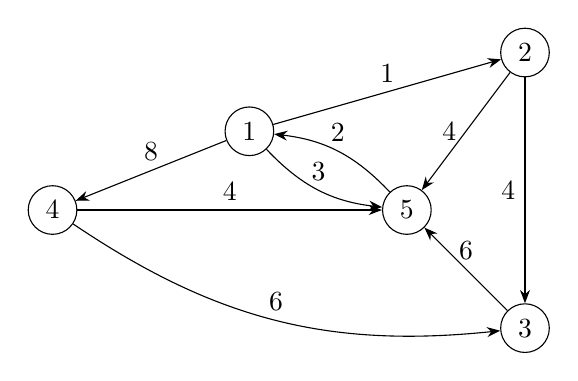
\begin{tikzpicture}
			\usetikzlibrary{arrows.meta}
%			\node[draw,circle] (v0)  at (0,  3.5)	{$6$};
			\node[draw,circle] (v1)  at (2.5,2.5)	{$1$};
			\node[draw,circle] (v2)  at (6,  3.5)	{$2$};
%			\node[draw,circle] (v3)  at (12, 3.5)	{$3$};
			\node[draw,circle] (v4)  at (0,1.5)	{$4$};
			\node[draw,circle] (v5)  at (4.5,1.5)	{$5$};
%			\node[draw,circle] (v6)  at (9,1.75)	{$6$};
%			\node[draw,circle] (v7)  at (12,1.75)	{$7$};
%			\node[draw,circle] (v8)  at (2.5,0)	{$6$};
			\node[draw,circle] (v9)  at (6,0)	{$3$};
%			\node[draw,circle] (v10) at (9,0)	{$7$};
%			\node[draw,circle] (v11) at (12,0)	{$11$};
			%
			\def\list {v1/v2/1, v1/v4/8, %v0/v1/6, v0/v2/4, v1/v5/3, v2/v3/6, v2/v6/8,
      v4/v5/4, %v4/v8/5, v8/v9/1,
      v9/v5/6%, v9/v10/4, v10/v7/7, v10/v11/2
      }  % list elements
			\foreach \u\v\weight in \list
			{	\draw[-Stealth] (\u) -- (\v) node [midway, above] {\weight};
			}
			\def\vertical {v2/v5/4, v2/v9/4%, v0/v4/3, v3/v7/7, v6/v10/1, v11/v7/2
      }  % list elements
			\foreach \u\v\weight in \vertical
			{	\draw[-Stealth] (\u) -- (\v) node [midway, left] {\weight};
			}
			
%      \draw[-Stealth] (v10) -- (v2) node [midway, above] {5};
      \path[-Stealth] (v5) edge[bend angle=20, bend right] node[above] {2} (v1);
      \path[-Stealth] (v1) edge[bend angle=20, bend right] node[above] {3} (v5);
      \path[-Stealth] (v4) edge[bend angle=20, bend right] node[above] {6} (v9);
		\end{tikzpicture}
		\caption{\label{example_graph}Der gerichtete, gewichtete Graph $G$. Die Zahlen an den Kanten definieren die Funktion $w\colon E(G)\to\mathbb N$ der Kantengewichte.}
	\end{center}
\end{figure}
\end{aufgabe}

\begin{aufgabe}[APSP-Algorithmen anpassen]
\ 
  \begin{enumerate}
    \item Beschreibe, wie der Algorithmus \textsc{LeyzorekAPSP} [Erickson, Abschnitt~9.6] modifiziert werden kann, um neben dem Array der Längen kürzester Wege außerdem ein Array von Vorgänger-Pointern zurückzugeben.
    Die Laufzeit soll weiterhin in $O(V^3 \log V)$ liegen.
    \item Beschreibe, wie der Algorithmus \textsc{FloydWarshall} [Erickson, Abschnitt~9.8] modifiziert werden kann, um neben dem Array der Längen kürzester Wege außerdem ein Array von Vorgänger-Pointern zurückzugeben.
    Die Laufzeit soll weiterhin in $O(V^3)$ liegen.
  \end{enumerate}
  \emph{Hinweis}: Das gesuchte Array \texttt{pred} ist ein zweidimensionales Array, das jedem Knoten-Paar $(u,v)$ einen Knoten \texttt{pred[u,v]} zuordnet. Hierbei soll \texttt{pred[u,v]} der Vorgänger-Knoten von $v$ auf einem kürzesten Weg von $u$ nach $v$ sein.
\end{aufgabe}

%\begin{aufgabe}
%  Die in der Vorlesung behandelten Algorithmen scheitern, sobald ein negativer Zyklus im Graph enthalten ist.
%  Sie können allerdings so modifiziert werden, dass sie auch im Falle von negativen Zyklen korrekte Längen kürzester Pfade berechnen.
%  Damit ist gemeint, dass im Fall, das entsprechende Array \texttt{dist} für ein Knotenpaar $u,v$ folgenden Wert enthalten soll:
%  \begin{itemize}
%  	\item Gibt es keinen $u$-$v$-Pfad im Graphen, dann soll $\texttt{dist}[u,v] = \infty$ sein.
%    \item Ist von $u$ ein negativer Zyklus erreichbar, von dem aus wiederum $v$ erreichbar ist, so soll $\texttt{dist}[u,v] = -\infty$ sein.
%    \item Andernfalls soll $\texttt{dist}[u,v]$ die Länge eines kürzesten $u$-$v$-Pfades angeben.
%  \end{itemize}
%  \begin{enumerate}
%    \item Zeige dies beispielhaft für den Floyd-Warshall-Algorithmus.
%    Beschreibe also, wie dieser modifiziert werden kann, um auch im Falle von negativen Zyklen korrekte Längen kürzester  Wege zu berechnen.
%    \item Zeige, dass der Floyd-Warshall-Algorithmus außerdem so modifiziert werden kann, dass er einen negativen Zyklus im Graphen zurückgibt, falls ein solcher existiert. Andernfalls soll weiterhin das Array der Längen kürzester Wege zurückgegeben werden.
%  \end{enumerate}
%\end{aufgabe}

\begin{aufgabe}[Mortys Labyrinth]
    Morty muss einen stabilisierten Plumbus aus dem Klappen\-spitzen-Labyrinth beschaffen.
    Er muss dazu mit Ricks interdimensionaler \textit{portal gun} das Labyrinth betreten, durch das Labyrinth zu einem Plumbus vordringen, anschließend den (instabilen) Plumbus durch das Labyrinth zu einem Fleeb bringen, um ihn zu stabilisieren, und schließlich wieder zurück zum ursprünglichen Portal, um nach Hause zurückzukehren.
    Plumbusse werden durch Fleeb-Saft stabilisiert, der von jedem Fleeb abgesondert wird, sobald er aus seinem Fleeb-Loch entfernt wird.
    Instabile Plumbusse explodieren, wenn sie von ihrer Aufbewahrungs-Einheit über 137 Flinks weit getragen werden.
    Zudem stinkt das Klappenspitzen-Labyrinth nach Furz, weshalb Morty so wenig Zeit wie möglich dort verbringen will.

    Rick hat Morty für diese Aufgabe eine detaillierte Karte des Labyrinths gegeben, die aus einem gerichteten Graphen $G = (V,E)$ mit nicht-negativen Kantengewichten besteht (diese geben die Abstände in Flinks an).
    Zusätzlich hat er ihm die Menge $P \subseteq V$ der Plumbus-Aufbewahrungseinheiten und die Menge $F \subseteq V$ der Fleeb-Löcher mitgeteilt.
    
    Morty hat nun die Aufgabe, einen Startknoten $s \in V$, eine Plumbus-Aufbewahrungseinheit $p \in P$ und ein Fleeb-Loch $f \in F$ zu finden, sodass die Länge eines kürzesten Wegs von $p$ nach $f$ höchstens 137 Flinks beträgt und die Länge eines kürzesten Wegs, der von $s$ zunächst über $p$ und dann über $f$ schließlich zurück zu $s$ führt, so kurz wie möglich ist.

    Beschreibe einen Algorithmus, um Mortys Problem zu lösen, und analysiere seine Laufzeit.
    Du darfst annehmen, dass eine Lösung existiert.
\end{aufgabe}

\end{document}
